\chapter{Технологический раздел}

В технологическом разделе выбраны и описаны средства реализации программного обеспечения и представлены детали его реализации.
В качестве языка программирования был выбран С++,~т.~к. он 
как он позволяет реализовать все алгоритмы, выбранные в результате проектирования, а также поддерживает все требуемые структуры данных. Для создания пользовательского интерфейса использовался фреймворк Qt,~т.~к. в нем присутствуют необходимые для этого инструменты, для задач визуализации --- библиотека SFML.

\section{Графический интерфейс программы}
На рисунке~\ref{fig:interface} представлен интерфейс программы. + описание
\begin{figure}[H]
	\centering
	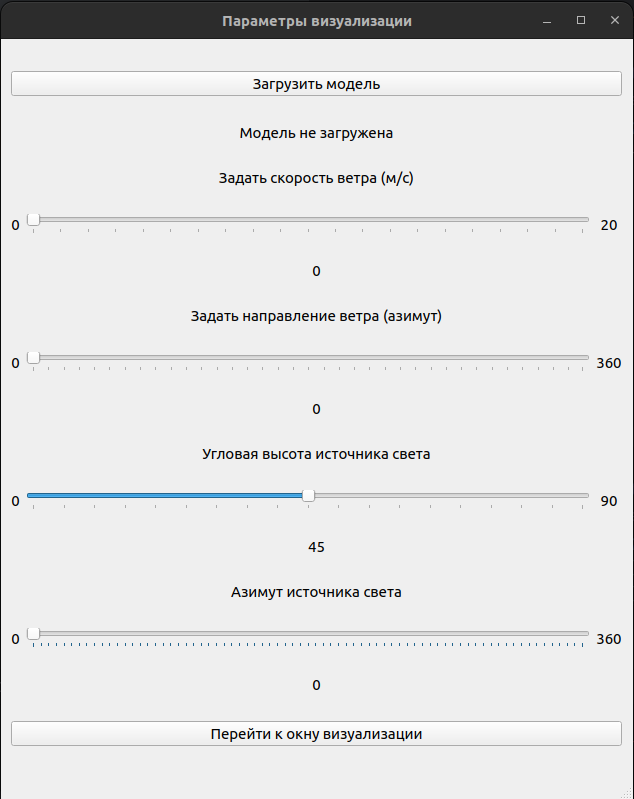
\includegraphics[width=1.0\textwidth, page=1]{assets/img/interface.png}   
	\caption{Интерфейс программы.}
	\label{fig:interface}
\end{figure}
\section{Реализация алгоритмов}

В листинге~\ref{lst:upd_voxels} представлен листинг функции изменения модели под влиянием ветра.
\newpage
\begin{lstlisting}[style=C, caption={Фунция изменения модели под влиянием ветра},label={lst:upd_voxels}]
public static void UpdateVoxelPhysics(
List<ModelVoxel> voxels,
Vector3D windForce,
double deltaTime,
bool isLowerLevelFixed)
{
	foreach (var voxel in voxels)
	{
		if (isLowerLevelFixed && (voxel.Level == 0)) continue;
		
		Vector3D displacement = voxel.CurrentCenter - voxel.OriginalCenter;
		Vector3D springForce = -displacement * voxel.SpringStiffness;
		Vector3D effectiveWind = windForce;
		
		voxel.Velocity += (springForce + effectiveWind) * deltaTime;
		voxel.Velocity *= voxel.SpringDamping;
		
		Point3D newCenter = voxel.CurrentCenter + voxel.Velocity * deltaTime;
		
		Vector3D totalDisplacement = newCenter - voxel.OriginalCenter;
		if (totalDisplacement.Length > MAX_DISPLACEMENT)
		{
			totalDisplacement.Normalize();
			totalDisplacement *= MAX_DISPLACEMENT;
			newCenter = voxel.OriginalCenter + totalDisplacement;
			voxel.Velocity *= 0.5; 
		}
		
		Vector3D movement = newCenter - voxel.CurrentCenter;
		voxel.CurrentCenter = newCenter;
		
		voxel.Bounds = new Rect3D(
		voxel.Bounds.X + movement.X,
		voxel.Bounds.Y + movement.Y,
		voxel.Bounds.Z + movement.Z,
		voxel.Bounds.SizeX,
		voxel.Bounds.SizeY,
		voxel.Bounds.SizeZ
		);
	}
}
\end{lstlisting}

\section{Модульное тестирование}

Для модульного тестирования был использован XUnit. Тестировались критически важные функции. Покрытие составило 20,4\%. В листинге ~\ref{lst:test_voxels} приведен пример тестов для функции отрисовки вокселей.
\newpage
\begin{lstlisting}[style=C, caption={Тест для функций отрисовки вокселей},label={lst:test_voxels}]

public class VoxelGeneratorTests
{
[Fact]
public void ModelVoxel_Initialization_CorrectCenters()
{
	var bounds = new Rect3D(0, 0, 0, 10, 10, 10);
	var voxel = new VoxelGenerator.ModelVoxel(bounds, 1);
	
	Assert.Equal(new Point3D(5, 5, 5), voxel.OriginalCenter);
	Assert.Equal(new Point3D(5, 5, 5), voxel.CurrentCenter);
}
[Fact]
public void TransformContainedModels_AppliesCorrectTransformation()
{
	var bounds = new Rect3D(0, 0, 0, 10, 10, 10);
	var voxel = new VoxelGenerator.ModelVoxel(bounds, 1);
	var model = new GeometryModel3D();
	voxel.ContainedModels.Add(model);
	
	voxel.CurrentCenter = new Point3D(10, 10, 10);
	voxel.TransformContainedModels();
	
	Assert.IsType<TranslateTransform3D>(model.Transform);
}
[Fact]
public void UpdateVoxelPhysics_ChangesVoxelVelocity()
{
	var voxel = new VoxelGenerator.ModelVoxel(new Rect3D(0, 0, 0, 10, 10, 10), 1)
	{
		SpringStiffness = 0.1,
		SpringDamping = 0.9
	};
	List<VoxelGenerator.ModelVoxel> voxels = new() { voxel };
	Vector3D windForce = new(1, 0, 0);
	
	VoxelGenerator.UpdateVoxelPhysics(voxels, windForce, 0.1, false);
	
	Assert.NotEqual(new Vector3D(0, 0, 0), voxel.Velocity);
}

\end{lstlisting}

\section*{Вывод}
В данном разделе были выбраны средства реализации программного обеспечения, были проведены модульные тесты, все тесты пройдены успешно. Покрытие программы модульными тестами составило 20.4\%.
